\documentclass[11pt,a4paper]{article}

\usepackage[T1]{fontenc}
\usepackage[utf8]{inputenc}
\usepackage[spanish,es-nodecimaldot]{babel}
\usepackage[a4paper,margin=2.35cm]{geometry}
\usepackage{lmodern}
\usepackage{microtype}
\usepackage{setspace}
\usepackage{parskip}
\usepackage{amsmath,amssymb,bm}
\usepackage{booktabs}
\usepackage{threeparttable}
\usepackage{tabularx}
\usepackage{longtable}
\usepackage{array}
\usepackage{multirow}
\usepackage{siunitx}
\usepackage{graphicx}
\usepackage{float}
\usepackage[section]{placeins}
\usepackage{subcaption}
\usepackage{xcolor}
\usepackage{enumitem}
\usepackage{fancyhdr}
\usepackage{titlesec}
\usepackage[hidelinks]{hyperref}

\graphicspath{{figures/}}
\onehalfspacing
\setlength{\parindent}{0pt}
\setlength{\parskip}{0.55em}
\setcounter{tocdepth}{2}
\sisetup{
  output-decimal-marker={,},
  group-separator={\,},
  group-minimum-digits=4,
  detect-all
}

\definecolor{navy}{HTML}{0D3B66}
\definecolor{ochre}{HTML}{C77D18}
\definecolor{brick}{HTML}{9A2D2D}
\definecolor{forest}{HTML}{2A6F4E}
\definecolor{lightgray}{HTML}{F2F3F4}

\hypersetup{
  colorlinks=true,
  linkcolor=navy,
  citecolor=navy,
  urlcolor=navy
}

\pagestyle{fancy}
\fancyhf{}
\lhead{\small QBART y riesgo cambiario de cola}
\rhead{\small Informe exploratorio v2}
\cfoot{\thepage}
\renewcommand{\headrulewidth}{0.4pt}

\titleformat{\section}
  {\Large\bfseries\color{navy}}{\thesection.}{0.55em}{}
\titleformat{\subsection}
  {\large\bfseries\color{navy}}{\thesubsection.}{0.55em}{}
\titleformat{\subsubsection}
  {\normalsize\bfseries\color{brick}}{\thesubsubsection.}{0.55em}{}

\newcolumntype{L}{>{\raggedright\arraybackslash}X}
\newcolumntype{R}{>{\raggedleft\arraybackslash}X}
\newcommand{\taup}[1]{\(\tau=#1\)}
\newcommand{\qbart}{\textsc{QBART}}
\newcommand{\qrf}{\textsc{QRF}}
\newcommand{\rw}{\textsc{RW}}
\newcommand{\pinball}{\mathcal{L}_{\tau}}

\begin{document}

\hypersetup{pageanchor=false}
\begin{titlepage}
\centering
\vspace*{1.2cm}
{\bfseries\Large PONTIFICIA UNIVERSIDAD CATÓLICA DEL PERÚ\par}
\vspace{0.45cm}
{\bfseries\large FACULTAD DE CIENCIAS SOCIALES\par}
\vspace{0.9cm}

\includegraphics[width=0.22\textwidth]{logo_pucp.jpg}
\vspace{0.9cm}

{\color{navy}\rule{\textwidth}{1.1pt}}
\vspace{0.55cm}
{\bfseries\LARGE
Pronóstico de percentiles extremos del tipo de cambio peruano
\par}
\vspace{0.3cm}
{\bfseries\Large
Metodología, especificación y resultados exploratorios de QBART
\par}
\vspace{0.55cm}
{\color{navy}\rule{\textwidth}{1.1pt}}

\vspace{1.2cm}
{\large Comparación sistemática con Quantile Random Forest y Random Walk\par}
\vspace{1.4cm}

\begin{tabular}{rl}
\textbf{Autora:} & Sinthya Bernabe Ortega \\
\textbf{Código:} & 20222834 \\
\textbf{Profesor:} & Jairo Flores \\
\textbf{Versión:} & Informe exploratorio v2 \\
\textbf{Fecha:} & 17 de julio de 2026 \\
\end{tabular}

\vfill
{\small Lima, Perú\par}
\end{titlepage}

\clearpage
\pagenumbering{roman}
\hypersetup{pageanchor=true}

\begin{abstract}
Este informe documenta de manera reproducible la evaluación exploratoria de
Bayesian Quantile Additive Regression Trees (\qbart) para pronosticar los
percentiles 5, 50 y 95 del retorno diario futuro del tipo de cambio nominal
sol/dólar. El experimento emplea 6\,832 observaciones entre marzo de 2000 y
junio de 2026, 46 predictores causales y una evaluación cronológica con
ventana móvil de 2\,520 observaciones. \qbart se estima con el kernel C++
oficial de BayesQArt y se compara, bajo la misma información y los mismos
orígenes, con Quantile Random Forest (\qrf), regresión cuantílica lineal y un
benchmark de Random Walk definido mediante cuantiles históricos.

La calibración causal corrige la marcada contracción de las colas del
\qbart crudo: la cobertura pasa de 0,162 a 0,045 para el percentil 5 y de
0,844 a 0,950 para el percentil 95. Sin embargo, \qrf mantiene una menor
pérdida pinball en los tres percentiles. Frente a \qrf, el \qbart calibrado
presenta pérdidas 21,4\%, 18,3\% y 16,9\% mayores para los percentiles 5,
50 y 95, respectivamente. Los tests de Diebold--Mariano rechazan igualdad
predictiva a favor de \qrf. Además, aunque \qbart supera el test de cobertura
incondicional de Kupiec luego de calibrarse, falla el test de cobertura
dinámica en ambas colas. El análisis temporal muestra una señal favorable
en 2026, pero insuficiente para revertir el resultado agregado.

En cuanto a los determinantes, la cola izquierda se asocia principalmente
con medidas de volatilidad y forma de la distribución reciente, mientras
que la cola derecha asigna mayor frecuencia a monedas internacionales,
reservas, DXY y aceleración de volatilidad. Estas frecuencias son señales
exploratorias de nacimientos de ramas aceptados, incluyendo burn-in, y no
deben interpretarse como probabilidades posteriores de inclusión.
\end{abstract}

\textbf{Palabras clave:} tipo de cambio, riesgo de cola, regresión
cuantílica, BART, QBART, Quantile Random Forest, pronóstico.

\textbf{Clasificación JEL:} C11, C14, C22, C53, F31, G17.

\newpage
\tableofcontents
\clearpage
\pagenumbering{arabic}

\section{Objetivo y preguntas del ejercicio}

El objetivo es evaluar si una especificación bayesiana no paramétrica
orientada directamente a cuantiles puede pronosticar la variabilidad extrema
del tipo de cambio peruano y revelar determinantes diferentes en el centro y
en las colas de la distribución condicional. El análisis se concentra en
tres objetos:

\begin{enumerate}[leftmargin=*]
  \item el percentil 5 del retorno futuro, asociado a movimientos extremos
  negativos del tipo de cambio expresado en soles por dólar;
  \item la mediana condicional, que sirve como referencia central; y
  \item el percentil 95, asociado a movimientos extremos positivos y, bajo
  esta convención, a depreciaciones fuertes del sol.
\end{enumerate}

La pregunta predictiva central es si \qbart puede igualar o superar a \qrf
y al Random Walk en pérdida pinball fuera de muestra. La pregunta económica
es si el conjunto de variables utilizado por los árboles cambia entre
\(\tau=0.05\), \(0.50\) y \(0.95\). Finalmente, se analiza si una buena
cobertura incondicional implica también estabilidad temporal de las
violaciones de los cuantiles.

\subsection{Criterio de comparación}

La comparación principal se realiza mediante pérdida pinball. Una menor
pérdida representa un mejor pronóstico. La cobertura es una condición
adicional: un percentil puede presentar cobertura cercana al valor nominal
y, aun así, ser poco informativo o demasiado ancho. Por ello, cobertura y
pinball se interpretan conjuntamente. \qrf constituye el benchmark de
aprendizaje automático más exigente; el Random Walk sirve como referencia
parsimoniosa y la regresión cuantílica permite medir cuánto aporta la
no linealidad.

\section{Diseño empírico}

\subsection{Variable objetivo}

Sea \(s_t\) el tipo de cambio nominal expresado en soles por dólar. El retorno
diario se expresa en puntos porcentuales. Para horizonte \(h=1\), la variable
objetivo disponible en la observación fechada en \(t\) es:

\begin{equation}
  y_{t+1} = 100\,\Delta \log(s_{t+1}).
\end{equation}

En el código, el retorno futuro se construye desplazando la respuesta una
observación hacia adelante. Los predictores de la fila \(t\) utilizan
únicamente información observada hasta \(t\). Una realización positiva
corresponde a un aumento del precio del dólar y, por tanto, a una
depreciación del sol.

\subsection{Muestra y partición cronológica}

Después de construir rezagos, transformaciones y estadísticas móviles, la
muestra contiene 6\,832 observaciones completas. No se realiza una división
aleatoria. El primer 60\% se reserva como bloque inicial de entrenamiento,
el siguiente 20\% como validación y el último 20\% como test.

\begin{table}[H]
\centering
\caption{Partición cronológica de la muestra}
\label{tab:sample}
\begin{threeparttable}
\begin{tabular}{lrrr}
\toprule
Bloque & Observaciones & Inicio & Fin \\
\midrule
Muestra completa & 6\,832 & 27/03/2000 & 02/06/2026 \\
Train inicial & 4\,099 & 27/03/2000 & 10/12/2015 \\
Validación & 1\,366 & 11/12/2015 & 05/03/2021 \\
Test & 1\,367 & 08/03/2021 & 02/06/2026 \\
\bottomrule
\end{tabular}
\begin{tablenotes}[flushleft]\footnotesize
\item La estimación efectiva utiliza una ventana móvil de las últimas 2\,520
observaciones disponibles. En el tuning se toman las últimas 2\,520
observaciones del bloque inicial de entrenamiento.
\end{tablenotes}
\end{threeparttable}
\end{table}

\subsection{Ventana móvil y bloques de reestimación}

En cada origen de reestimación \(b\), los modelos emplean:

\begin{equation}
  \mathcal{I}_b =
  \{t_b-2520,\ldots,t_b-1\},
\end{equation}

donde \(t_b\) es la primera fecha del bloque. El test se divide en 23 bloques
de hasta 60 observaciones. Los modelos se reestiman al inicio de cada bloque
y producen los cuantiles para las observaciones del bloque. Este esquema
reduce el costo computacional, mantiene la dirección temporal y aplica el
mismo conjunto de información a todos los métodos.

El diseño no equivale a una reestimación diaria. Dentro de cada bloque, los
parámetros permanecen fijos hasta el siguiente origen. Esta aproximación es
común a \qbart, \qrf y regresión cuantílica, por lo que conserva la equidad
comparativa, pero puede reducir la capacidad de adaptación ante quiebres
que ocurran dentro de los 60 días.

\subsection{Predictores}

El conjunto final contiene 46 variables. La Tabla~\ref{tab:predictors}
resume su construcción.

\begin{table}[H]
\centering
\caption{Grupos de predictores}
\label{tab:predictors}
\small
\begin{tabularx}{\textwidth}{p{3.6cm}p{1.2cm}L}
\toprule
Grupo & Número & Variables y transformación \\
\midrule
Condiciones globales y tasas & 9 &
VIX, BAA--Treasury spread, tasa de Estados Unidos, NFCI, yield to
worst, term premia a 1, 5 y 10 años, y EMBIG Perú. \\
Política y mercado cambiario & 4 &
Variación del VIX, diferencial de tasas Perú--Estados Unidos,
intervención del BCRP e indicador de intervención faltante. \\
Precios y monedas & 18 &
Cambios logarítmicos de reservas, oro, cobre, zinc, plata, S\&P 500,
MSCI emergentes, DXY y monedas internacionales y regionales. WTI usa
diferencias de \(\operatorname{asinh}\) porque puede tomar valores no
positivos. \\
Dinámica del retorno & 7 &
Cinco rezagos, valor absoluto y cuadrado del retorno más reciente. \\
Volatilidad y forma & 8 &
Desviaciones estándar de 5, 20 y 60 días, EWMA con
\(\lambda=0.94\), media absoluta de 20 días, asimetría de 20 días,
curtosis de 60 días y ratio de volatilidad 5/60. \\
\midrule
\textbf{Total} & \textbf{46} & \\
\bottomrule
\end{tabularx}
\end{table}

Las variables móviles incluyen la observación \(t\), que está disponible al
pronosticar \(t+1\). Los valores faltantes de intervención se sustituyen por
cero, pero se incorpora un indicador de ausencia para distinguir ``sin
intervención'' de ``dato no reportado''. Las transformaciones eliminan
observaciones iniciales hasta disponer de las ventanas necesarias.

\subsection{Prevención de look-ahead}

El procedimiento impone cuatro restricciones:

\begin{enumerate}[leftmargin=*]
  \item la respuesta siempre corresponde al retorno futuro;
  \item el tuning usa únicamente train y validación;
  \item la evaluación final no modifica hiperparámetros usando resultados
  del test; y
  \item la calibración de un bloque utiliza solo errores observados en
  validación y en bloques de test ya realizados.
\end{enumerate}

El checkpoint incluye un hash de datos, fechas, configuración, semillas y
versión del paquete para impedir la mezcla accidental de resultados
provenientes de especificaciones diferentes.

\section{Modelos}

\subsection{Random Walk cuantílico}

El benchmark denominado Random Walk supone que el retorno es impredecible
condicionalmente y que la distribución relevante puede aproximarse con la
distribución empírica reciente. Su pronóstico es:

\begin{equation}
  \widehat q_{\tau,t}^{RW}
  =
  Q_{\tau}\{y_s:s\in\mathcal{I}_t\}.
\end{equation}

En sentido estricto, se trata de un benchmark de cuantiles históricos bajo
retornos tipo caminata aleatoria, no de fijar el retorno pronosticado en
cero. Es difícil de superar porque adapta automáticamente la escala a la
volatilidad de la ventana, aunque no utiliza información condicional.

\subsection{Regresión cuantílica lineal}

Para cada \(\tau\), la regresión cuantílica estima:

\begin{equation}
  \widehat{\bm\beta}_{\tau}
  =
  \arg\min_{\bm\beta}
  \sum_{t\in\mathcal{I}_b}
  \rho_{\tau}
  \left(y_{t+1}-\bm x_t^{\prime}\bm\beta\right),
\end{equation}

donde
\begin{equation}
  \rho_{\tau}(u)=u\left[\tau-\mathbf{1}(u<0)\right].
\end{equation}

La especificación utiliza los 46 predictores. Su ventaja es la transparencia;
su limitación es que restringe los efectos marginales a ser lineales y
aditivos. Como cada percentil se estima por separado, las predicciones se
reordenan por observación para evitar cruces.

\subsection{Quantile Random Forest}

\qrf utiliza la estructura de Random Forest para estimar una distribución
condicional ponderada. Si \(w_i(\bm x)\) es el peso inducido por la frecuencia
con la que la observación \(i\) comparte nodos terminales con \(\bm x\),
entonces:

\begin{equation}
  \widehat F(y\mid\bm x)
  =
  \sum_{i=1}^{n}w_i(\bm x)\mathbf{1}(y_i\leq y),
\end{equation}

y el cuantil se obtiene mediante:

\begin{equation}
  \widehat q_{\tau}^{QRF}(\bm x)
  =
  \inf\{y:\widehat F(y\mid\bm x)\geq\tau\}.
\end{equation}

La principal fortaleza es que un único bosque proporciona todos los
percentiles y captura interacciones y no linealidades sin imponer una forma
paramétrica \cite{meinshausen2006}. El tuning emplea una pérdida normalizada
por el Random Walk y pondera más las colas, evitando que la escala de la
mediana domine la selección.

\subsection{Bayesian Quantile Additive Regression Trees}

\subsubsection{Función cuantílica}

\qbart representa el cuantil condicional como suma de árboles:

\begin{equation}
  q_{\tau}(\bm x)
  =
  G_{\tau}(\bm x)
  =
  \sum_{j=1}^{m}g(\bm x;T_{j,\tau},M_{j,\tau}),
\end{equation}

donde \(T_{j,\tau}\) es la estructura del árbol y \(M_{j,\tau}\) contiene
los parámetros de sus nodos terminales. A diferencia de un BART de media,
cada \(\tau\) tiene su propio ensamble, por lo que variables y particiones
pueden cambiar entre centro y colas.

La implementación de Kindo et al.\ utiliza una representación
normal--exponencial de la distribución Laplace asimétrica
\cite{kindo2016}. Condicional en la variable latente \(\nu_i\):

\begin{equation}
  y_i
  =
  G_{\tau}(\bm x_i)
  +
  \vartheta_{1,\tau}\nu_i
  +
  \sqrt{\phi\,\vartheta_{2,\tau}^{2}\nu_i}\,z_i,
  \qquad z_i\sim N(0,1),
\end{equation}

con:

\begin{equation}
  \vartheta_{1,\tau}
  =
  \frac{1-2\tau}{\tau(1-\tau)},
  \qquad
  \vartheta_{2,\tau}^{2}
  =
  \frac{2}{\tau(1-\tau)}.
\end{equation}

Esta mezcla permite actualizar árboles, nodos, latentes y escala mediante
MCMC. Los priors estructurales siguen la lógica regularizadora de BART:
la probabilidad de dividir un nodo a profundidad \(d\) es
\(\alpha(1+d)^{-\beta}\), con \(\alpha=0.95\) y \(\beta=2\)
\cite{chipman2010}.

\subsubsection{Motor oficial y transformación de predictores}

La corrida utiliza el kernel C++ oficial BayesQArt, fijado al commit
\texttt{3f83a7f}. El motor local en R se conserva únicamente como
implementación experimental y no participa en los resultados. Esta decisión
se tomó porque el kernel local empleaba una secuencia de movimientos y
ratios de aceptación simplificados que no garantizaban la misma posterior.

Antes de ingresar a \qbart, cada predictor se transforma mediante su función
de distribución empírica en la ventana de entrenamiento. Esta transformación
monótona preserva el orden y hace que los cortes equidistantes del paquete
se aproximen a cortes por cuantiles. Los valores de test se mapean usando
exclusivamente la distribución del entrenamiento.

\subsubsection{Reordenamiento de cuantiles}

Como los tres ensambles se estiman por separado, pueden producir cruces. Se
aplica reordenamiento por fila:

\begin{equation}
  \left(
  \widehat q_{0.05,t},
  \widehat q_{0.50,t},
  \widehat q_{0.95,t}
  \right)
  \leftarrow
  \operatorname{sort}
  \left(
  \widehat q_{0.05,t},
  \widehat q_{0.50,t},
  \widehat q_{0.95,t}
  \right),
\end{equation}

siguiendo la idea de rearrangement monotónico de
\cite{chernozhukov2010}.

\section{Tuning y especificación seleccionada}

\subsection{Tuning por percentil}

La selección de \qbart se realiza separadamente para cada \(\tau\):

\begin{equation}
  \widehat{\theta}_{\tau}
  =
  \arg\min_{\theta\in\Theta}
  \sum_{t\in\mathcal V}
  \rho_{\tau}
  \left(
  y_{t+1}-\widehat q_{\tau,t}(\theta)
  \right),
\end{equation}

donde \(\mathcal V\) es el bloque de validación. Esto corrige una limitación
de la versión anterior, que promediaba las pérdidas de tres percentiles y
daba peso implícitamente mayor a la mediana.

La grilla exploratoria considera:

\begin{equation}
  \kappa\in\{0.5,1,2\},\quad
  m\in\{50,100\},\quad
  n_{\min}\in\{5,15\},\quad
  d_{\max}=3.
\end{equation}

Cada configuración usa dos semillas, 200 iteraciones de burn-in y 300
iteraciones retenidas en tuning. La corrida fuera de muestra usa 1\,000 de
burn-in y 2\,000 posteriores.

\begin{table}[H]
\centering
\caption{Hiperparámetros seleccionados por percentil}
\label{tab:qbart-tuning}
\begin{tabular}{lrrrrr}
\toprule
Percentil & \(\kappa\) & Árboles & \(n_{\min}\) & Profundidad & Pinball validación \\
\midrule
5  & 0,5 & 50 & 5  & 3 & 0,04386 \\
50 & 0,5 & 50 & 15 & 3 & 0,11580 \\
95 & 2,0 & 50 & 15 & 3 & 0,03806 \\
\bottomrule
\end{tabular}
\end{table}

Los tres percentiles seleccionan 50 árboles. En esta grilla, aumentar a 100
árboles no mejora la validación. El percentil 5 prefiere nodos más pequeños
y menor shrinkage, mientras que el percentil 95 selecciona mayor
\(\kappa\) y nodos mínimos de 15 observaciones.

\subsection{Tuning de QRF}

\qrf se ajusta de manera comparable con:

\begin{equation}
  n_{\text{tree}}\in\{300,500\},\quad
  mtry\in\{6,15\},\quad
  n_{\min}\in\{5,15\}.
\end{equation}

El criterio es un promedio de pérdidas relativas al Random Walk con pesos
\((0.4,0.2,0.4)\) para los percentiles 5, 50 y 95. La especificación
seleccionada utiliza 300 árboles, \(mtry=6\) y \(n_{\min}=15\). Sus pérdidas
de validación son 0,03519, 0,10669 y 0,03179. Por tanto, la ventaja de \qrf
ya era visible antes de observar el test: el mejor \qbart era 24,6\% peor
en el percentil 5, 8,5\% peor en la mediana y 19,7\% peor en el percentil
95.

\section{Calibración causal de QBART}

\subsection{Motivación}

Tanto en simulaciones como en la aplicación real, el \qbart crudo contrae
los extremos hacia el centro: el percentil 5 queda demasiado alto y el
percentil 95 demasiado bajo. Para separar error de localización de error de
forma, se aplica una corrección aditiva basada en errores pasados.

Sea:

\begin{equation}
  e_{\tau,s}=y_s-\widehat q^{raw}_{\tau,s}.
\end{equation}

Al inicio del bloque \(b\), se calcula:

\begin{equation}
  \widehat\delta_{\tau,b}
  =
  Q_{\tau}
  \left(
  \{e_{\tau,s}:s<t_b\}_{\text{últimos 500}}
  \right),
\end{equation}

y:

\begin{equation}
  \widehat q^{cal}_{\tau,t}
  =
  \widehat q^{raw}_{\tau,t}
  +
  \widehat\delta_{\tau,b}.
\end{equation}

El historial inicial procede de predicciones de validación generadas con un
modelo entrenado únicamente en train. Después se incorporan bloques de test
ya observados. No se emplea información futura.

\begin{figure}[H]
\centering
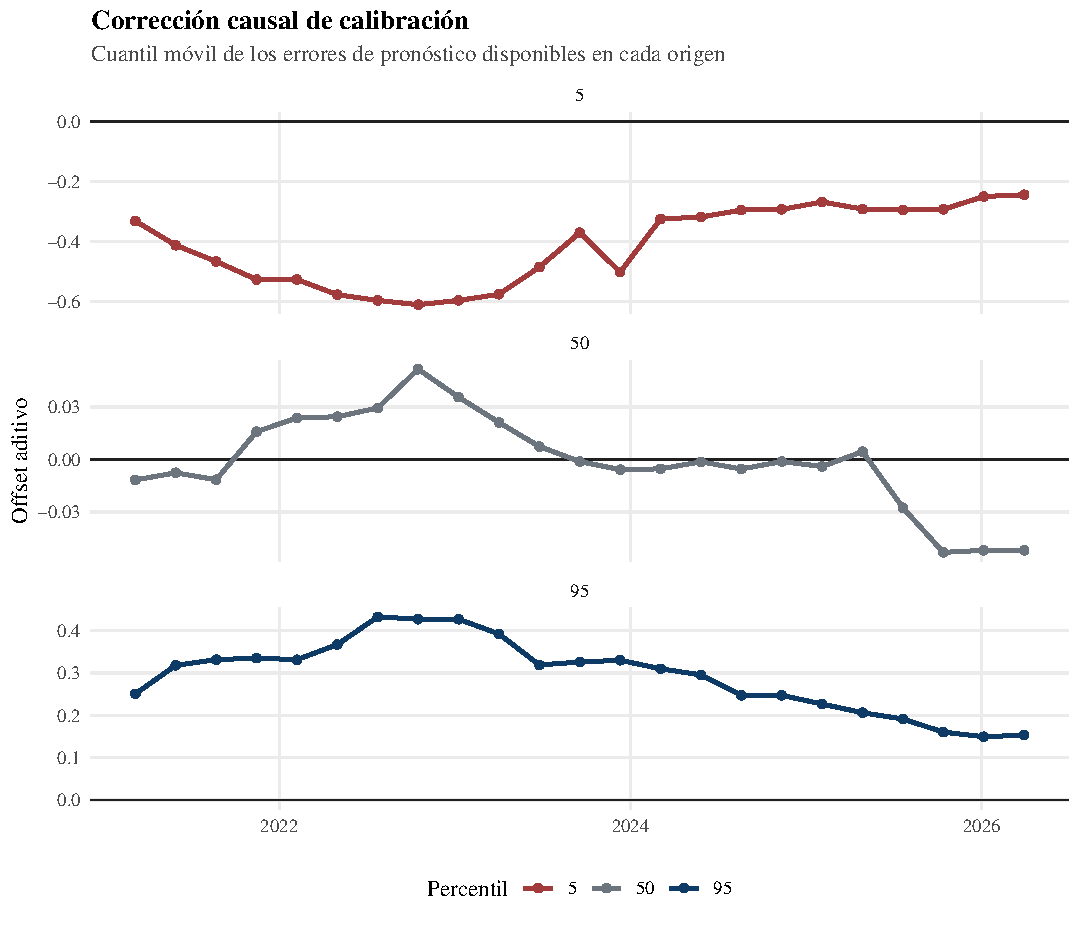
\includegraphics[width=0.92\textwidth]{qbart_report_calibration.pdf}
\caption{Evolución de los offsets de calibración.}
\label{fig:calibration}
\end{figure}

La Figura~\ref{fig:calibration} evidencia no estacionariedad. El ajuste del
percentil 5 alcanza aproximadamente \(-0.61\) y termina en \(-0.24\); el del
percentil 95 alcanza \(+0.43\) y termina cerca de \(+0.15\). La mediana
requiere correcciones mucho menores. Esta evolución anticipa que una ventana
de calibración fija puede ser demasiado lenta ante cambios de régimen.

\section{Métricas y pruebas}

\subsection{Pérdida pinball}

Para observaciones de test \(\mathcal T\):

\begin{equation}
  \widehat L_{\tau}
  =
  \frac{1}{|\mathcal T|}
  \sum_{t\in\mathcal T}
  \rho_{\tau}
  \left(y_t-\widehat q_{\tau,t}\right).
\end{equation}

Es una regla de scoring propia para cuantiles. El ratio
\(\widehat L_{\tau}^{m}/\widehat L_{\tau}^{RW}\) menor que uno indica que el
método \(m\) supera al Random Walk.

\subsection{Cobertura}

\begin{equation}
  \widehat C_{\tau}
  =
  \frac{1}{|\mathcal T|}
  \sum_{t\in\mathcal T}
  \mathbf{1}
  \left(y_t\leq\widehat q_{\tau,t}\right).
\end{equation}

Un cuantil está calibrado incondicionalmente si
\(\widehat C_{\tau}\approx\tau\).

\subsection{Kupiec, DQ y Diebold--Mariano}

El test de Kupiec contrasta cobertura incondicional usando una razón de
verosimilitudes binomial \cite{kupiec1995}. El test Dynamic Quantile (DQ)
emplea:

\begin{equation}
  H_t=\mathbf{1}(y_t\leq\widehat q_{\tau,t})-\tau
\end{equation}

y prueba conjuntamente constante y cuatro rezagos mediante:

\begin{equation}
  DQ
  =
  (\bm X^{\prime}\bm H)^{\prime}
  \left[
  \tau(1-\tau)\bm X^{\prime}\bm X
  \right]^{-1}
  (\bm X^{\prime}\bm H),
\end{equation}

con distribución asintótica \(\chi^2\) bajo la nula
\cite{englemanganelli2004}. Finalmente, Diebold--Mariano compara las pérdidas
diarias de \qbart y \qrf usando una varianza HAC
\cite{dieboldmariano1995}. Una diferencia media positiva implica mayor
pérdida de \qbart.

\section{Ejercicios de validación previos}

\subsection{Revisión del sampler}

La primera implementación local actualizaba la variable latente una vez por
iteración, simplificaba ratios Metropolis--Hastings y ejecutaba una sola
propuesta estructural por árbol. Debido a que estas diferencias podían
alterar la distribución objetivo, se sustituyó por el kernel oficial. El
motor local quedó bloqueado para resultados de investigación.

\subsection{Simulation gate}

Se generó una función no lineal heterocedástica con cuantiles verdaderos
conocidos. La muestra completa del gate usa 400 observaciones de ajuste, 400
de calibración y 1\,200 de test. \qbart emplea 100 árboles, 1\,000
iteraciones de burn-in y 1\,500 posteriores.

\begin{table}[H]
\centering
\caption{Simulation gate completo}
\label{tab:simulation}
\small
\begin{tabular}{lrrrr}
\toprule
Percentil & Métrica & QBART crudo & QBART calibrado & QRF \\
\midrule
\multirow{2}{*}{5}
 & Pinball   & 0,07654 & 0,06420 & 0,06058 \\
 & Cobertura & 0,13583 & 0,04583 & 0,05500 \\
\midrule
\multirow{2}{*}{50}
 & Pinball   & 0,24402 & 0,24425 & 0,19810 \\
 & Cobertura & 0,49917 & 0,51833 & 0,49917 \\
\midrule
\multirow{2}{*}{95}
 & Pinball   & 0,08568 & 0,06439 & 0,05883 \\
 & Cobertura & 0,82500 & 0,95583 & 0,95833 \\
\bottomrule
\end{tabular}
\end{table}

\begin{figure}[H]
\centering
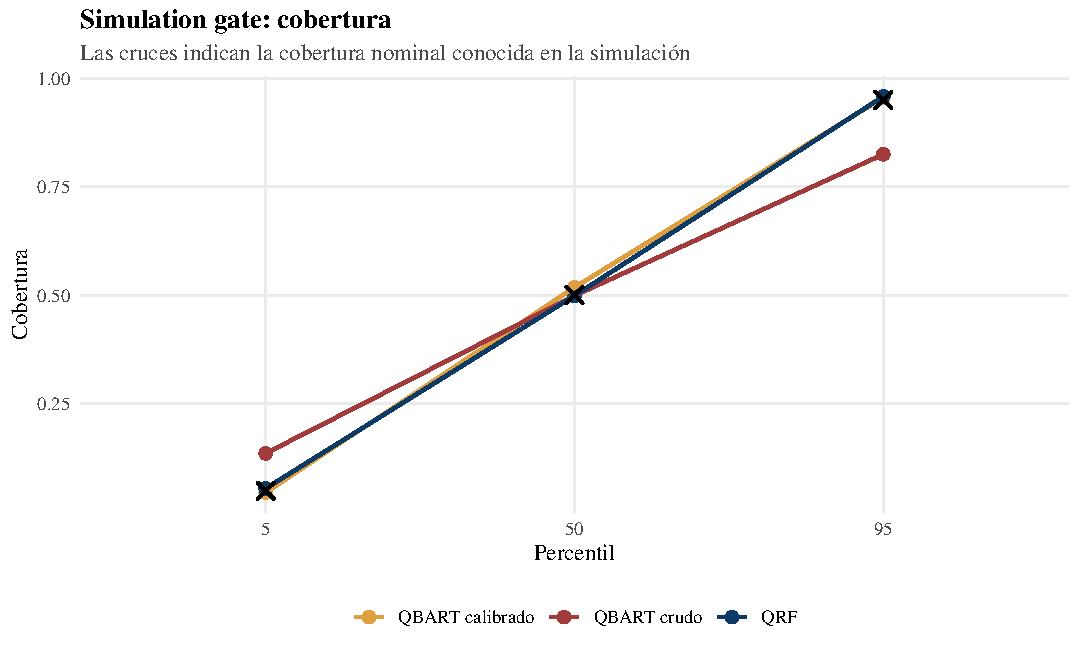
\includegraphics[width=0.82\textwidth]{qbart_report_simulation.pdf}
\caption{Cobertura de los métodos en el simulation gate.}
\label{fig:simulation}
\end{figure}

El ejercicio reproduce el sesgo hacia el centro incluso cuando la función
generadora es conocida. Cadenas más largas mejoran estabilidad, pero no
eliminan la contracción. La calibración corrige cobertura y deja a \qbart
entre 6,0\% y 9,4\% detrás de \qrf en las colas. Esto anticipa que aumentar
solamente el número de iteraciones no garantiza superar a \qrf.

\subsection{Pruebas de software}

Se incorporaron pruebas de:

\begin{itemize}[leftmargin=*]
  \item disponibilidad obligatoria del motor oficial;
  \item hiperparámetros diferenciados por percentil;
  \item preservación del orden bajo rank transform;
  \item dimensiones, finitud y ausencia de cruces;
  \item calibración monotónica; y
  \item capacidad del test DQ para detectar cobertura incorrecta.
\end{itemize}

\section{Resultados fuera de muestra}

\subsection{Pérdida pinball}

\begin{table}[H]
\centering
\caption{Pérdida pinball fuera de muestra}
\label{tab:score}
\begin{threeparttable}
\begin{tabular}{lrrrrr}
\toprule
Percentil & Random Walk & Reg. cuantílica & QRF & QBART crudo & QBART calibrado \\
\midrule
5  & 0,05548 & 0,04853 & \textbf{0,04721} & 0,07255 & 0,05730 \\
50 & 0,14642 & 0,14844 & \textbf{0,14634} & 0,17272 & 0,17317 \\
95 & 0,04961 & 0,04551 & \textbf{0,04459} & 0,06416 & 0,05212 \\
\bottomrule
\end{tabular}
\begin{tablenotes}[flushleft]\footnotesize
\item Menor es mejor. El valor en negrita identifica el mejor método por
percentil.
\end{tablenotes}
\end{threeparttable}
\end{table}

\begin{figure}[H]
\centering
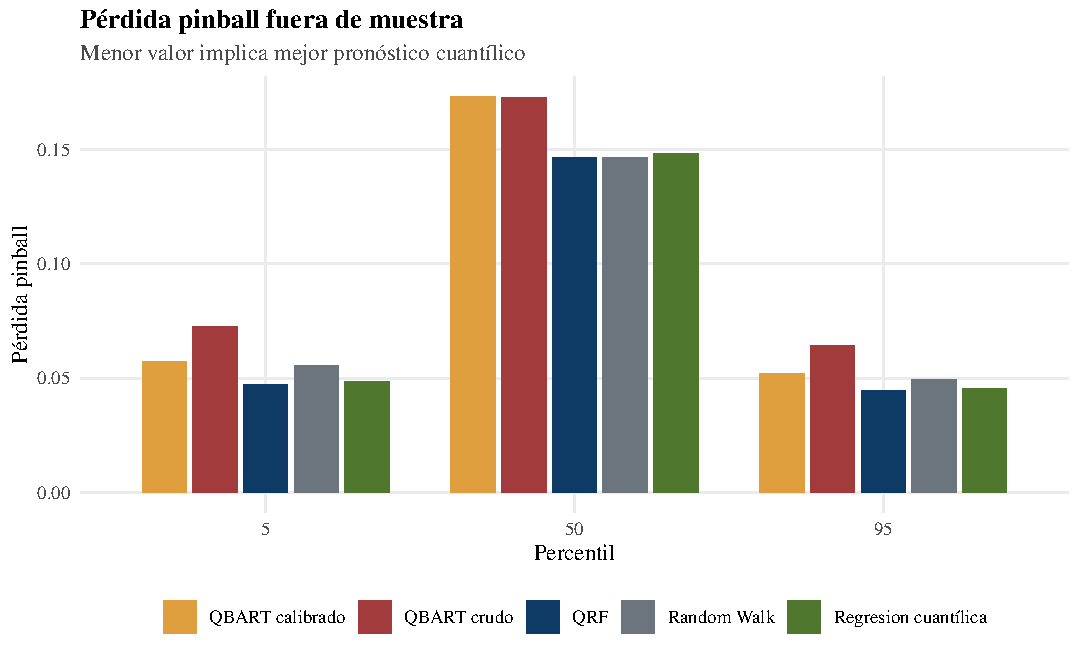
\includegraphics[width=0.9\textwidth]{qbart_report_scores.pdf}
\caption{Comparación de pérdida pinball.}
\label{fig:scores}
\end{figure}

\qrf obtiene la menor pérdida en los tres percentiles. La calibración reduce
la pérdida de \qbart en 21,0\% para el percentil 5 y en 18,8\% para el 95,
pero no mejora la mediana. Frente a \qrf, las brechas del \qbart calibrado
son:

\begin{equation}
  21.4\%\quad(\tau=0.05),\qquad
  18.3\%\quad(\tau=0.50),\qquad
  16.9\%\quad(\tau=0.95).
\end{equation}

El \qbart calibrado tampoco supera al Random Walk: sus ratios son 1,033,
1,183 y 1,051. La regresión cuantílica queda muy cerca de \qrf en las colas,
lo que sugiere que parte importante de la señal puede capturarse de forma
lineal con el conjunto ampliado de predictores.

\subsection{Cobertura}

\begin{table}[H]
\centering
\caption{Cobertura empírica}
\label{tab:coverage}
\small
\begin{tabular}{lrrrrrr}
\toprule
\(\tau\) & Nominal & Random Walk & Reg. cuantílica & QRF & QBART crudo & QBART calibrado \\
\midrule
0,05 & 0,050 & 0,087 & 0,064 & 0,059 & 0,162 & \textbf{0,045} \\
0,50 & 0,500 & 0,530 & 0,503 & 0,525 & 0,512 & \textbf{0,503} \\
0,95 & 0,950 & 0,922 & 0,936 & 0,945 & 0,844 & \textbf{0,950} \\
\bottomrule
\end{tabular}
\end{table}

\begin{figure}[H]
\centering
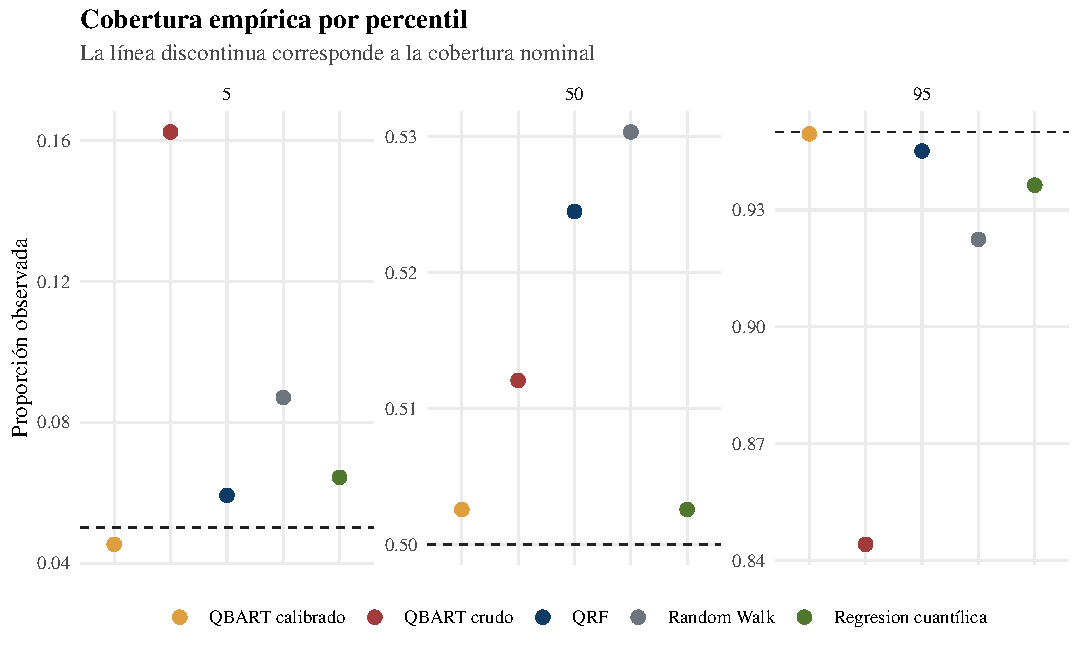
\includegraphics[width=0.94\textwidth]{qbart_report_coverage.pdf}
\caption{Cobertura observada y nominal.}
\label{fig:coverage}
\end{figure}

La calibración alcanza una cobertura promedio más próxima a la nominal que
\qrf. Sin embargo, este resultado no contradice el ranking de pinball:
una corrección aditiva puede ajustar la frecuencia promedio de violaciones
sin mejorar suficientemente la localización condicional de cada pronóstico.

\subsection{Backtests corregidos}

\begin{table}[H]
\centering
\caption{Tests de cobertura y precisión}
\label{tab:tests}
\small
\begin{tabular}{llrrrr}
\toprule
Método & \(\tau\) & \(p\) Kupiec & \(p\) DQ & DM vs. QRF & \(p\) DM \\
\midrule
\multirow{3}{*}{QRF}
 & 0,05 & 0,127 & 0,052 & -- & -- \\
 & 0,50 & 0,070 & 0,227 & -- & -- \\
 & 0,95 & 0,416 & 0,149 & -- & -- \\
\midrule
\multirow{3}{*}{QBART crudo}
 & 0,05 & \(<10^{-50}\) & \(<10^{-70}\) & 6,844 & \(<10^{-11}\) \\
 & 0,50 & 0,372 & 0,043 & 9,670 & \(<10^{-21}\) \\
 & 0,95 & \(<10^{-47}\) & \(<10^{-69}\) & 6,309 & \(<10^{-9}\) \\
\midrule
\multirow{3}{*}{QBART calibrado}
 & 0,05 & 0,424 & 0,001 & 4,918 & \(<10^{-6}\) \\
 & 0,50 & 0,850 & 0,071 & 9,617 & \(<10^{-21}\) \\
 & 0,95 & 0,936 & \(<10^{-5}\) & 4,944 & \(<10^{-6}\) \\
\bottomrule
\end{tabular}
\end{table}

\qrf no es rechazado al 5\% por Kupiec ni por DQ. El percentil 5 tiene
\(p=0.052\) en DQ y merece seguimiento, pero no cruza el umbral convencional.
El \qbart calibrado supera Kupiec en los tres casos y falla DQ en ambas
colas. En consecuencia, la cobertura promedio correcta oculta clustering de
violaciones y cambios de régimen.

Las estadísticas Diebold--Mariano son positivas y altamente significativas.
La diferencia media diaria de pérdida de \qbart calibrado respecto a \qrf es
0,01009, 0,02682 y 0,00753 para los percentiles 5, 50 y 95. La hipótesis de
igual precisión se rechaza a favor de \qrf.

\subsection{Comparación con la versión anterior}

\begin{table}[H]
\centering
\caption{Cambio de desempeño respecto a la exploración anterior}
\label{tab:old-new}
\begin{tabular}{lrrr}
\toprule
Percentil & QBART anterior & QBART v2 calibrado & Cambio \\
\midrule
5  & 0,06122 & 0,05730 & \(-6,4\%\) \\
50 & 0,14651 & 0,17317 & \(+18,2\%\) \\
95 & 0,05379 & 0,05212 & \(-3,1\%\) \\
\bottomrule
\end{tabular}
\end{table}

Las colas mejoran en términos absolutos respecto a la versión local anterior.
No obstante, \qrf también mejora aproximadamente 8,1\% y 8,3\% en las colas,
por lo que la brecha relativa no se cierra. La comparación es indicativa:
la incorporación de estadísticas móviles elimina once observaciones
iniciales adicionales y modifica ligeramente la muestra.

\section{Estabilidad temporal}

\subsection{Resultados anuales}

\begin{table}[H]
\centering
\caption{Ratio anual de pérdida QBART calibrado/QRF}
\label{tab:yearly}
\begin{tabular}{lrrr}
\toprule
Año & Percentil 5 & Mediana & Percentil 95 \\
\midrule
2021 & 1,241 & 1,138 & 1,233 \\
2022 & 1,270 & 1,131 & 1,145 \\
2023 & 1,240 & 1,171 & 1,208 \\
2024 & 1,240 & 1,222 & 1,161 \\
2025 & 1,198 & 1,319 & 1,227 \\
2026 & \textbf{0,901} & 1,169 & \textbf{0,929} \\
\bottomrule
\end{tabular}
\end{table}

\begin{figure}[H]
\centering
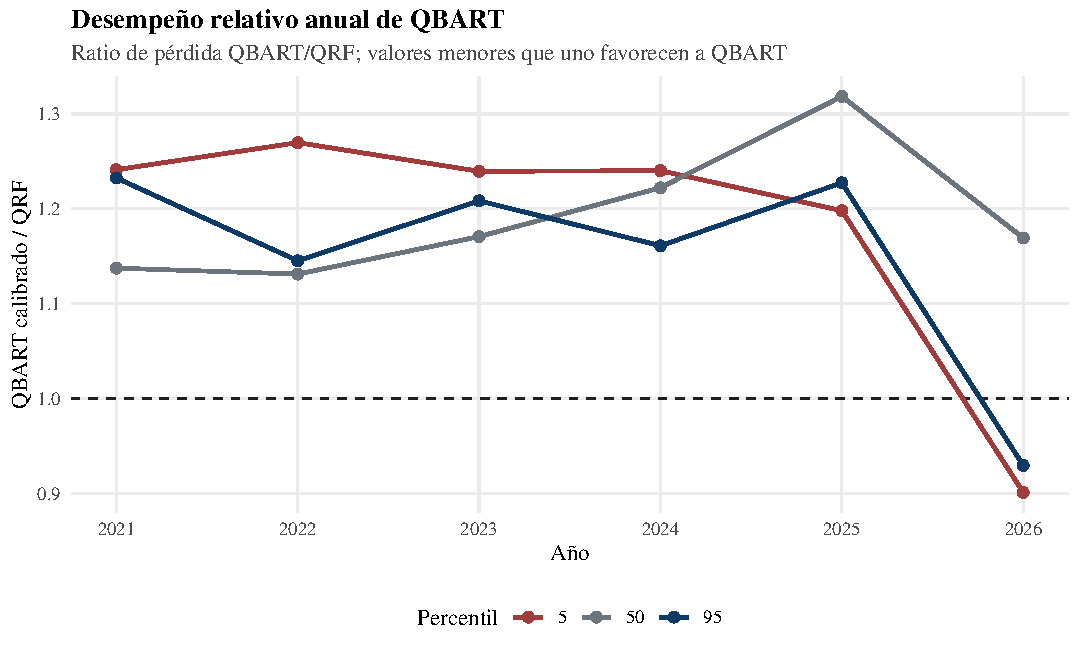
\includegraphics[width=0.9\textwidth]{qbart_report_yearly_ratio.pdf}
\caption{Evolución anual del desempeño relativo.}
\label{fig:yearly}
\end{figure}

\qbart pierde en ambas colas durante 2021--2025. En 2026 presenta ratios
menores que uno: 0,901 y 0,929 para los percentiles 5 y 95. La evidencia es
prometedora para el régimen reciente, pero se basa en 109 observaciones y no
revierte el resultado completo. La mediana permanece detrás de \qrf en todos
los años.

\subsection{Resultados por bloque}

\begin{figure}[H]
\centering
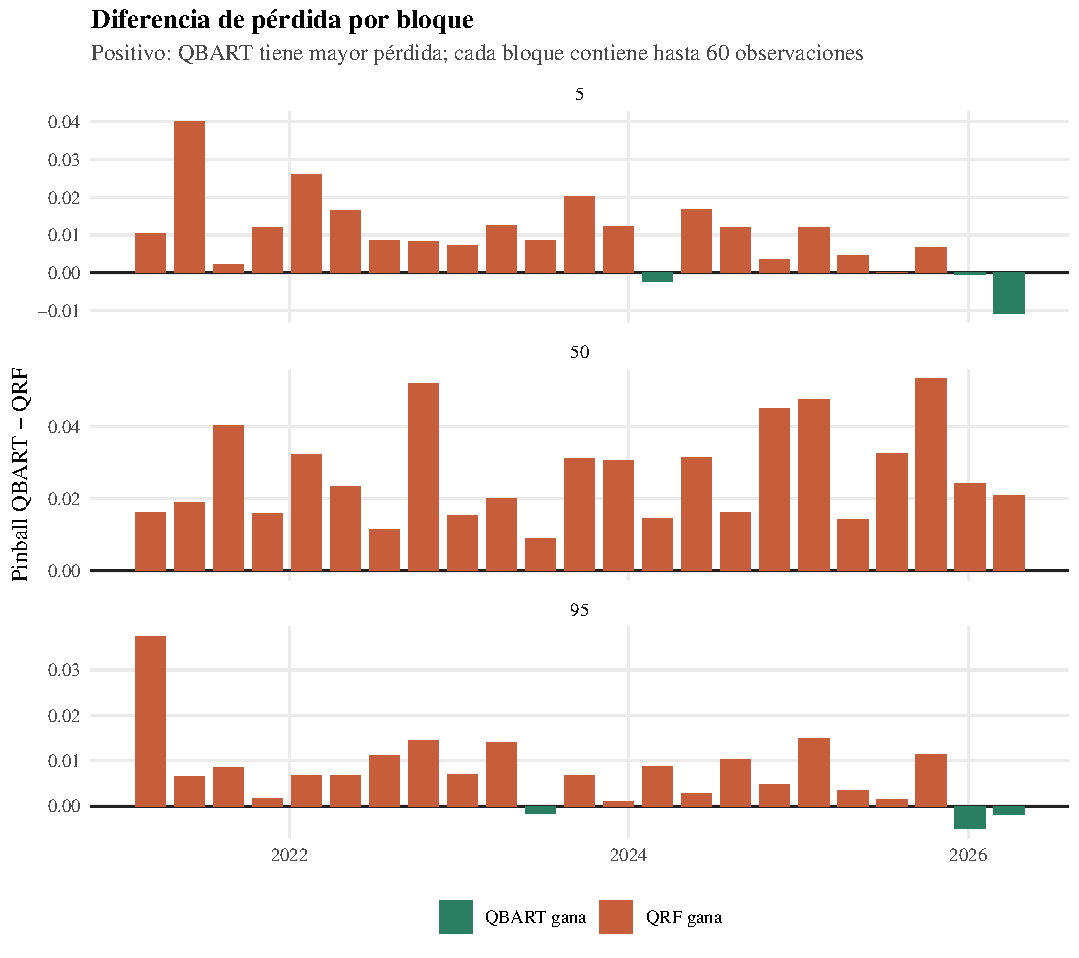
\includegraphics[width=0.95\textwidth]{qbart_report_block_difference.pdf}
\caption{Diferencia de pérdida QBART menos QRF por bloque.}
\label{fig:blocks}
\end{figure}

\qbart gana solo 3 de 23 bloques en el percentil 5, 0 de 23 en la mediana y
3 de 23 en el percentil 95. Los mejores bloques de cola se concentran hacia
el final de la muestra. La correlación entre la diferencia de pérdida y la
volatilidad móvil de 20 días es cercana a 0,08 en ambas colas; por tanto, la
desventaja no puede atribuirse únicamente a episodios de alta volatilidad.

\section{Determinantes por percentil}

\subsection{Definición de la medida}

El paquete oficial retorna la variable empleada cada vez que se acepta un
nacimiento de rama durante MCMC. Para cada percentil se cuenta:

\begin{equation}
  I_{j,\tau}
  =
  \frac{
  \#\{\text{nacimientos aceptados que usan }x_j\}
  }{
  \#\{\text{nacimientos aceptados}\}
  }.
\end{equation}

Esta medida incluye burn-in, no registra negativamente las podas y no
promedia el uso de variables sobre árboles posteriores almacenados. Por ello:

\begin{itemize}[leftmargin=*]
  \item no es una probabilidad posterior de inclusión;
  \item no mide efecto causal;
  \item puede estar influida por la frecuencia de propuestas aceptadas; y
  \item debe interpretarse como señal exploratoria de uso estructural.
\end{itemize}

La comparación entre percentiles es parcialmente favorecida porque los tres
modelos seleccionan 50 árboles y usan la misma longitud de cadena.

\subsection{Ranking principal}

\begin{table}[H]
\centering
\caption{Principales señales de uso por percentil}
\label{tab:importance}
\small
\begin{tabular}{lrlrlr}
\toprule
\multicolumn{2}{c}{Percentil 5} &
\multicolumn{2}{c}{Mediana} &
\multicolumn{2}{c}{Percentil 95} \\
\cmidrule(lr){1-2}\cmidrule(lr){3-4}\cmidrule(lr){5-6}
Variable & Frec. & Variable & Frec. & Variable & Frec. \\
\midrule
\texttt{mean\_abs\_ret\_20} & 0,066 &
\texttt{d\_oro} & 0,088 &
\texttt{d\_eur} & 0,070 \\
\texttt{vol\_sd\_20} & 0,062 &
\texttt{d\_mxn} & 0,076 &
\texttt{d\_gbp} & 0,062 \\
\texttt{skew\_ret\_20} & 0,062 &
\texttt{kurt\_ret\_60} & 0,072 &
\texttt{vol\_ratio\_5\_60} & 0,062 \\
\texttt{ret\_lag\_4} & 0,058 &
\texttt{ret\_lag\_1} & 0,060 &
\texttt{d\_cny} & 0,049 \\
\texttt{d\_clp} & 0,054 &
\texttt{interv\_bcrp} & 0,054 &
\texttt{d\_rin} & 0,041 \\
\texttt{kurt\_ret\_60} & 0,054 &
\texttt{d\_vix} & 0,051 &
\texttt{d\_dxy} & 0,041 \\
\texttt{d\_cobre} & 0,051 &
\texttt{tp\_5y} & 0,049 &
\texttt{ret\_lag\_4} & 0,041 \\
\texttt{ret\_lag\_5} & 0,051 &
\texttt{d\_zinc} & 0,046 &
\texttt{interv\_bcrp} & 0,037 \\
\bottomrule
\end{tabular}
\end{table}

\begin{figure}[H]
\centering
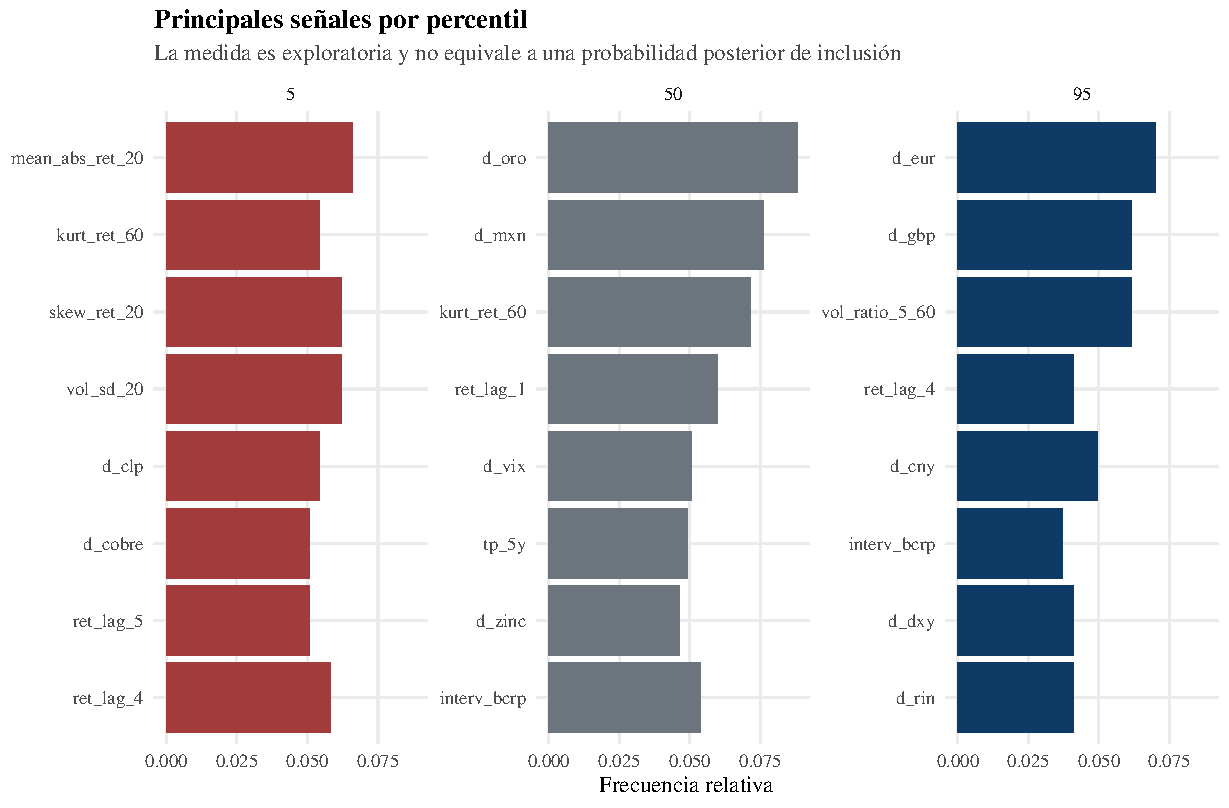
\includegraphics[width=0.94\textwidth]{qbart_report_importance_top.pdf}
\caption{Ocho señales principales en cada percentil.}
\label{fig:importance-top}
\end{figure}

\begin{figure}[H]
\centering
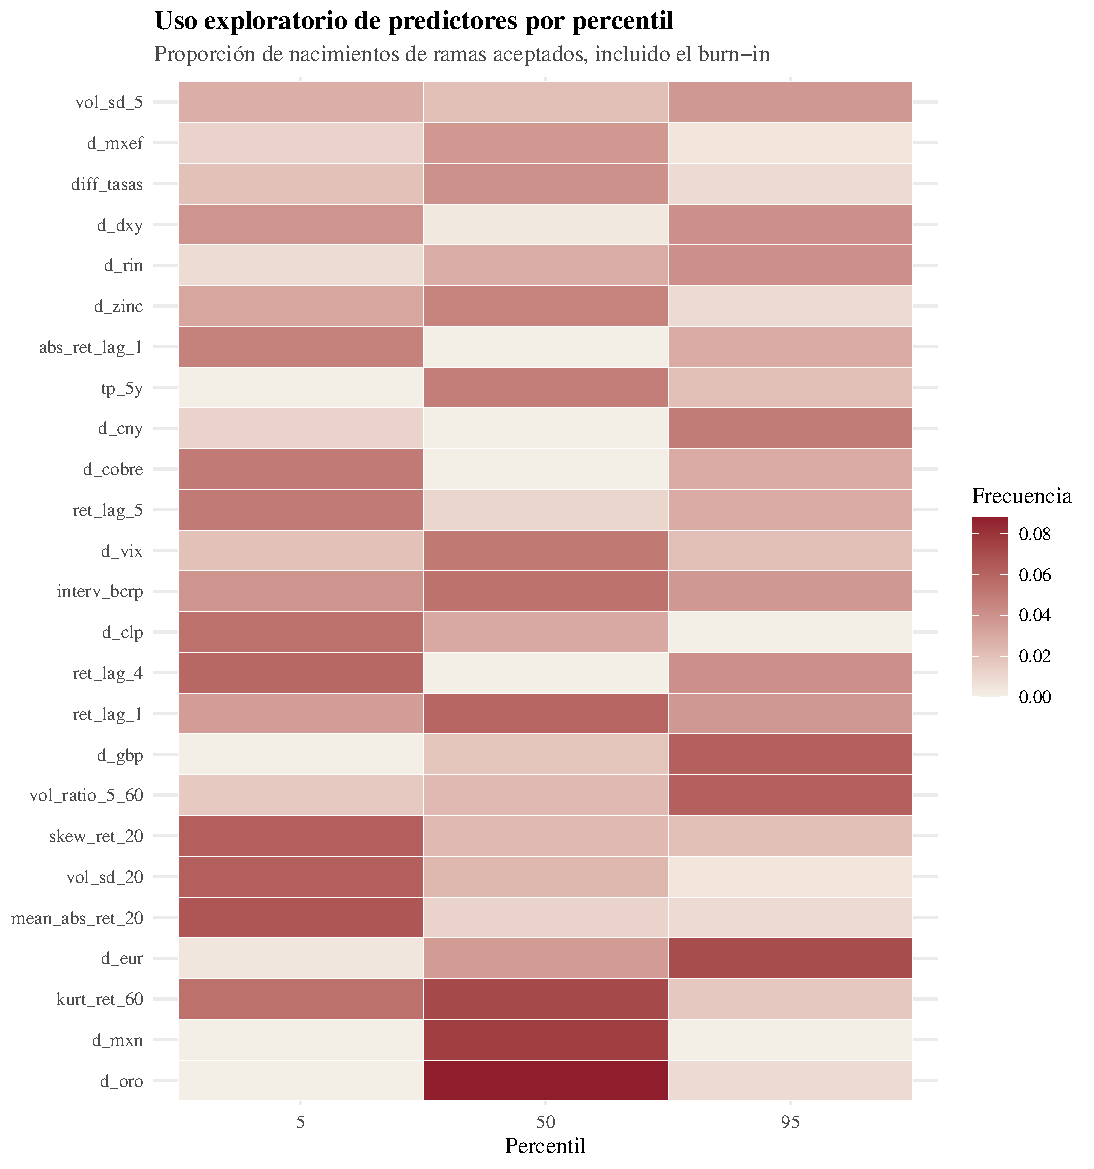
\includegraphics[width=\textwidth,height=0.76\textheight,keepaspectratio]{qbart_report_importance_heatmap.pdf}
\caption{Mapa de frecuencias absolutas para la unión de variables principales.}
\label{fig:importance-heatmap}
\end{figure}

\subsection{Interpretación de la cola izquierda}

La cola izquierda está dominada por medidas de variabilidad y forma:
media absoluta de retornos, volatilidad de 20 días, asimetría de 20 días y
curtosis de 60 días. También aparecen rezagos 4 y 5. El patrón sugiere que
los movimientos extremos negativos dependen de persistencia y acumulación de
volatilidad, más que de una única noticia contemporánea.

Entre las variables externas destacan CLP, cobre, plata, WTI y CHF. El peso
de CLP y cobre es coherente con exposición regional y de commodities. La
intervención del BCRP también aparece entre las diez primeras variables,
pero su frecuencia no debe interpretarse causalmente: la intervención es
endógena a presiones cambiarias y puede funcionar como indicador de estrés y
como respuesta amortiguadora simultáneamente.

\subsection{Interpretación del centro}

La mediana asigna mayor frecuencia a oro, MXN, curtosis de 60 días, retorno
reciente, intervención del BCRP, variación del VIX y term premium a cinco
años. Este conjunto es más heterogéneo y combina factores globales,
regionales y persistencia del retorno.

La importancia central no debe utilizarse como denominador mecánico cuando
es cercana a cero. Ratios cola/centro muy grandes, por ejemplo para DXY o
S\&P 500, pueden reflejar un denominador diminuto. Es preferible comparar
diferencias absolutas y estabilidad entre semillas.

\subsection{Interpretación de la cola derecha}

La cola derecha presenta mayor frecuencia en EUR, GBP, CNY, DXY, reservas y
el ratio de volatilidad 5/60. Bajo la convención soles por dólar, esta es la
cola asociada a depreciaciones extremas del sol. El patrón combina:

\begin{enumerate}[leftmargin=*]
  \item un componente de dólar y monedas internacionales;
  \item capacidad de intervención, aproximada por reservas;
  \item aceleración de volatilidad de corto plazo; y
  \item persistencia del retorno mediante rezagos.
\end{enumerate}

La intervención aparece nuevamente entre las variables principales. El VIX
en nivel tiene una frecuencia relativamente mayor en las colas que en el
centro, mientras que su variación diaria aparece más en la mediana. Esto
podría indicar que el régimen de riesgo global importa más que una variación
aislada para los eventos extremos.

\subsection{Asimetrías relevantes}

La comparación sugiere asimetrías económicamente plausibles:

\begin{itemize}[leftmargin=*]
  \item la cola izquierda enfatiza acumulación de volatilidad, asimetría,
  commodities y monedas regionales;
  \item la cola derecha enfatiza monedas globales, DXY, reservas y aceleración
  de volatilidad;
  \item intervención y dinámica rezagada aparecen en centro y colas; y
  \item las variables de volatilidad son importantes en ambas colas, pero con
  horizontes distintos: 20 días en la izquierda y 5/60 en la derecha.
\end{itemize}

Estas diferencias responden a la pregunta de investigación en sentido
exploratorio: los árboles construyen particiones diferentes por percentil.
No obstante, una afirmación definitiva requiere una medida posterior de
inclusión o importancia por permutación con incertidumbre.

\section{Ejercicios adicionales de análisis}

\subsection{Ensamble diagnóstico QBART--QRF}

Se calculó, solo como diagnóstico ex post, el peso \(w\) que minimiza la
pérdida de:

\begin{equation}
  \widehat q_{\tau}^{ens}
  =
  w\widehat q_{\tau}^{QRF}
  +(1-w)\widehat q_{\tau}^{QBART}.
\end{equation}

\begin{table}[H]
\centering
\caption{Ensamble diagnóstico ex post}
\label{tab:ensemble}
\begin{tabular}{lrr}
\toprule
Percentil & Peso óptimo de QRF & Mejora sobre QRF \\
\midrule
5  & 0,92 & 0,334\% \\
50 & 1,00 & 0,000\% \\
95 & 0,95 & 0,037\% \\
\bottomrule
\end{tabular}
\end{table}

Incluso con pesos elegidos mirando el test, el ensamble asigna casi toda la
masa a \qrf y genera mejoras económicamente despreciables. Por ello, un
promedio simple no resolvería la brecha actual.

\subsection{Concentración de señales}

Las diez variables principales concentran 54,5\% de los nacimientos
aceptados en el percentil 5, 57,3\% en la mediana y 47,7\% en el percentil
95. La cola derecha está algo menos concentrada, consistente con un conjunto
más diverso de canales internacionales.

\subsection{Evaluación de régimen}

La ventaja reciente de \qbart no se explica linealmente por la volatilidad
de 20 días: la correlación entre diferencia de pérdida y volatilidad es
aproximadamente 0,07--0,08. Esto sugiere que la fuente de heterogeneidad
puede involucrar composición de choques, relaciones no lineales o la
adaptación de los offsets, no solo la magnitud de la volatilidad.

\section{Limitaciones}

\begin{enumerate}[leftmargin=*]
  \item \textbf{Exploración MCMC.} Se utilizan 1\,000 iteraciones de burn-in
  y 2\,000 posteriores. Son más que un smoke test, pero menos que la
  configuración completa de 3\,000 y 5\,000.

  \item \textbf{Ausencia de draws en la interfaz oficial.} El paquete devuelve
  medias posteriores de predicción, no draws guardados. No pueden calcularse
  ESS, \(\widehat R\), intervalos posteriores ni estabilidad de funciones
  cuantílicas sin modificar C++.

  \item \textbf{Importancia imperfecta.} La frecuencia de nacimientos
  aceptados incluye burn-in y no equivale a inclusión posterior.

  \item \textbf{Distribución Laplace asimétrica.} La mezcla ALD facilita MCMC,
  pero puede inducir una forma de error demasiado restrictiva. La fuerte
  contracción de colas aparece también en simulación.

  \item \textbf{Reestimación en bloques.} Los modelos no se actualizan dentro
  de cada bloque de 60 observaciones.

  \item \textbf{Calibración aditiva.} El offset corrige localización promedio,
  pero no utiliza covariables ni modela explícitamente cambios en dispersión.

  \item \textbf{Timing de publicación.} Las transformaciones son causales en
  índice temporal, pero una versión final debe documentar lags de publicación
  y horarios de cierre de cada serie.

  \item \textbf{Intervención endógena.} Su frecuencia en árboles no identifica
  un efecto causal del BCRP.

  \item \textbf{Un solo horizonte.} Los resultados corresponden a un día y no
  necesariamente se extienden a horizontes semanales o mensuales.
\end{enumerate}

\section{Agenda para mejorar QBART}

\subsection{Prioridad 1: calibración dinámica}

Antes de una corrida completa se recomienda:

\begin{enumerate}[leftmargin=*]
  \item reconstruir las predicciones de validación y guardarlas;
  \item comparar ventanas de calibración de 125, 250 y 500 observaciones;
  \item estimar offsets separados por régimen de volatilidad;
  \item evaluar Adaptive Conformal Inference para actualizar cobertura
  objetivo; y
  \item seleccionar la regla exclusivamente con un backtest prequential de
  validación.
\end{enumerate}

Este ejercicio requiere reestimar solo tres modelos de validación y después
reutiliza las predicciones crudas. Su costo estimado es 15--25 minutos, muy
inferior a repetir la evaluación completa.

\subsection{Prioridad 2: mejorar la distribución de error}

La corrección necesaria de aproximadamente \(-0.41\) en la cola izquierda y
\(+0.29\) en la derecha indica un problema estructural de escala. Conviene
comparar:

\begin{itemize}[leftmargin=*]
  \item una Laplace asimétrica generalizada;
  \item mezclas con colas tipo Student-\(t\);
  \item BART distribucional con escala dependiente de \(\bm x\); y
  \item un modelo conjunto de varios cuantiles con restricción de no cruce.
\end{itemize}

\subsection{Prioridad 3: sparsity y selección de variables}

Con 46 predictores, el prior uniforme de variables puede diluir señal. Una
extensión DART o Dirichlet sobre probabilidades de split permitiría
concentrar masa en variables relevantes. Como alternativa, se puede realizar
preselección anidada por percentil usando únicamente train y validación.

\subsection{Prioridad 4: inferencia posterior e importancia robusta}

Debe modificarse el kernel C++ para guardar:

\begin{itemize}[leftmargin=*]
  \item predicciones por draw;
  \item \(\phi\), tamaño y profundidad de árboles;
  \item tasas de aceptación por movimiento;
  \item conteos de variables por draw posterior, excluyendo burn-in; y
  \item estado de los árboles para warm starts.
\end{itemize}

Con ello podrían calcularse intervalos, ESS, \(\widehat R\), probabilidades
de inclusión y estabilidad entre cadenas. Para determinantes, también se
recomienda importancia por permutación medida directamente en incremento de
pinball, repetida por percentil y bloque temporal.

\subsection{Prioridad 5: ventanas y regímenes}

La señal favorable en 2026 justifica comparar ventanas de 1\,000, 1\,500 y
2\,520 observaciones y ponderación exponencial. La selección debe realizarse
en backtests de validación, no mirando el test. También conviene reportar
resultados en submuestras de estrés, intervención intensa y alta volatilidad.

\subsection{Prioridad 6: eficiencia computacional}

La corrida exploratoria utilizó aproximadamente un núcleo lógico y tardó
seis horas. La versión completa no debe lanzarse secuencialmente. Se propone:

\begin{enumerate}[leftmargin=*]
  \item paralelizar configuraciones y semillas de tuning en 6--8 workers;
  \item paralelizar los tres percentiles dentro de cada bloque;
  \item mantener los bloques secuenciales para respetar la información;
  \item guardar checkpoints también durante tuning; y
  \item registrar tiempos, memoria, semillas y commit en cada ajuste.
\end{enumerate}

La evaluación por bloque podría acelerarse aproximadamente tres veces,
porque contiene tres ajustes \qbart independientes.

\subsection{Criterio para autorizar la corrida completa}

La corrida completa solo debería ejecutarse si una nueva especificación
cumple simultáneamente en validación:

\begin{enumerate}[leftmargin=*]
  \item cobertura dentro de \(\pm 0.02\) en ambos extremos;
  \item no rechazo de DQ al 5\%;
  \item pinball no mayor a 1,05 veces el de \qrf en cada cola;
  \item estabilidad en al menos dos semillas; y
  \item mejora en más de la mitad de los bloques de validación.
\end{enumerate}

\section{Conclusiones}

El experimento permite separar dos dimensiones. En calibración
incondicional, la versión v2 de \qbart funciona: corrige la cobertura de
colas hasta valores muy próximos a 0,05 y 0,95. En precisión condicional,
\qrf es superior: tiene menor pinball en los tres percentiles, supera los
backtests dinámicos y gana la mayoría de los bloques. La diferencia es
estadísticamente significativa y un ensamble ex post asigna entre 92\% y
100\% del peso a \qrf.

La principal lección metodológica es que cobertura promedio no basta. Los
offsets corrigen el nivel de los cuantiles, pero no su dinámica. El rechazo
de DQ en las colas y las variaciones anuales muestran que \qbart necesita una
calibración más adaptativa o una distribución de error más flexible.

La exploración de determinantes sí revela perfiles diferenciados. La cola
izquierda concentra medidas de volatilidad persistente, asimetría y
commodities; la derecha enfatiza monedas globales, DXY, reservas y
aceleración de volatilidad. La intervención del BCRP aparece de manera
recurrente. Estos resultados son hipótesis económicas valiosas, pero aún no
constituyen inferencia posterior ni causal.

En consecuencia, no se recomienda aumentar mecánicamente árboles y draws.
La siguiente etapa debe mejorar calibración dinámica, flexibilidad de escala,
sparsity e inferencia de importancia. Solo después de superar un nuevo gate
de validación tiene sentido asumir el costo de la corrida completa.

\appendix

\section{Reproducibilidad}

\subsection{Archivos principales}

\begin{longtable}{p{0.36\textwidth}p{0.56\textwidth}}
\toprule
Archivo & Contenido \\
\midrule
\endfirsthead
\toprule
Archivo & Contenido \\
\midrule
\endhead
\texttt{QBART\_riesgo\_de\_cola.R} &
Pipeline completo de datos, tuning, evaluación, calibración y resultados. \\
\texttt{notebooks/qbart\_adapter.R} &
Interfaz segura al kernel oficial y transformación de predictores. \\
\texttt{src/qbart\_features.R} &
Construcción causal de respuesta y 46 predictores. \\
\texttt{src/qbart\_workflow.R} &
Pinball, cobertura, tuning, calibración, Kupiec, DQ y DM. \\
\texttt{tests/qbart\_simulation\_gate.R} &
Simulación heterocedástica con cuantiles conocidos. \\
\texttt{tests/test\_qbart\_components.R} &
Pruebas de interfaz, monotonicidad y backtests. \\
\texttt{scripts/}\newline\texttt{build\_qbart\_report\_assets.R} &
Generación reproducible de figuras y tablas del presente informe. \\
\bottomrule
\end{longtable}

\subsection{Comandos}

\begin{verbatim}
Rscript --vanilla scripts/install_qbart_deps.R
Rscript --vanilla tests/test_qbart_components.R
Rscript --vanilla tests/qbart_simulation_gate.R

$env:QBART_MODE="exploracion"
$env:QBART_WINDOW_OBS="2520"
$env:QBART_REESTIMATION_STEP="60"
Rscript --vanilla QBART_riesgo_de_cola.R

Rscript --vanilla scripts/build_qbart_report_assets.R
\end{verbatim}

\section{Lista completa de predictores}

\small
\begin{longtable}{p{0.28\textwidth}p{0.66\textwidth}}
\toprule
Grupo & Variables \\
\midrule
\endfirsthead
\toprule
Grupo & Variables \\
\midrule
\endhead
Niveles &
\texttt{vix}, \texttt{baa10y}, \texttt{tasa\_usa}, \texttt{nfci},
\texttt{yield\_to\_worst}, \texttt{tp\_1y}, \texttt{tp\_5y},
\texttt{tp\_10y}, \texttt{embig\_peru}. \\
Política y tasas &
\texttt{d\_vix}, \texttt{diff\_tasas}, \texttt{interv\_bcrp},
\texttt{interv\_bcrp\_missing}. \\
Precios y monedas &
\texttt{d\_rin}, \texttt{d\_oro}, \texttt{d\_cobre},
\texttt{d\_zinc}, \texttt{d\_plata}, \texttt{d\_spx},
\texttt{d\_mxef}, \texttt{d\_dxy}, \texttt{d\_jpy},
\texttt{d\_chf}, \texttt{d\_eur}, \texttt{d\_gbp},
\texttt{d\_clp}, \texttt{d\_cop}, \texttt{d\_mxn},
\texttt{d\_brl}, \texttt{d\_cny}, \texttt{d\_wti}. \\
Rezagos &
\texttt{ret\_lag\_1}, \texttt{ret\_lag\_2},
\texttt{ret\_lag\_3}, \texttt{ret\_lag\_4},
\texttt{ret\_lag\_5}, \texttt{abs\_ret\_lag\_1},
\texttt{sq\_ret\_lag\_1}. \\
Volatilidad y forma &
\texttt{vol\_sd\_5}, \texttt{vol\_sd\_20}, \texttt{vol\_sd\_60},
\texttt{vol\_ewma\_094}, \texttt{mean\_abs\_ret\_20},
\texttt{skew\_ret\_20}, \texttt{kurt\_ret\_60},
\texttt{vol\_ratio\_5\_60}. \\
\bottomrule
\end{longtable}
\normalsize

\begin{thebibliography}{99}

\bibitem{chernozhukov2010}
Chernozhukov, V., Fernández-Val, I. y Galichon, A. (2010).
Quantile and probability curves without crossing.
\textit{Econometrica}, 78(3), 1093--1125.

\bibitem{chipman2010}
Chipman, H., George, E. y McCulloch, R. (2010).
BART: Bayesian additive regression trees.
\textit{The Annals of Applied Statistics}, 4(1), 266--298.

\bibitem{dieboldmariano1995}
Diebold, F. y Mariano, R. (1995).
Comparing predictive accuracy.
\textit{Journal of Business \& Economic Statistics}, 13(3), 253--263.

\bibitem{englemanganelli2004}
Engle, R. y Manganelli, S. (2004).
CAViaR: Conditional autoregressive value at risk by regression quantiles.
\textit{Journal of Business \& Economic Statistics}, 22(4), 367--381.

\bibitem{kindo2016}
Kindo, B., Wang, H., Hanson, T. y Peña, E. (2016).
Bayesian quantile additive regression trees.
\textit{arXiv preprint arXiv:1607.02676}.

\bibitem{koenkerbassett1978}
Koenker, R. y Bassett, G. (1978).
Regression quantiles.
\textit{Econometrica}, 46(1), 33--50.

\bibitem{kupiec1995}
Kupiec, P. (1995).
Techniques for verifying the accuracy of risk measurement models.
\textit{The Journal of Derivatives}, 3(2), 73--84.

\bibitem{meeserogoff1983}
Meese, R. y Rogoff, K. (1983).
Empirical exchange rate models of the seventies: Do they fit out of sample?
\textit{Journal of International Economics}, 14(1--2), 3--24.

\bibitem{meinshausen2006}
Meinshausen, N. (2006).
Quantile regression forests.
\textit{Journal of Machine Learning Research}, 7, 983--999.

\end{thebibliography}

\end{document}
